\documentclass{llncs}
\usepackage{llncsdoc}
\usepackage{mathpartir}
\usepackage{amsmath}
\usepackage{amssymb} 
%\usepackage{amsthm}
\usepackage{ stmaryrd }
%\usepackage{cite}
%\renewcommand{\citepunct}{,\,} % IEEEtran wants to use ],\,[ for this but that looks dumb...

\newcommand{\atlam}{@$\lambda$}

% Generic
\newcommand{\bindin}[2]{#1;~#2}
\newcommand{\pipe}{~\text{\large $\vert$}~}
\newcommand{\splat}[3]{#1_{#2};\ldots;#1_{#3}}
\newcommand{\splatC}[3]{#1_{#2}~~~~\cdots~~~~#1_{#3}}
\newcommand{\splatTwo}[4]{#1_{#3}#2_{#3},~\ldots~, #1_{#4}#2_{#4}}
\newcommand{\substn}[2]{[#1]#2}
\newcommand{\subst}[3]{\substn{#1/#2}{#3}}
\newcommand{\entails}[2]{#1 \vdash #2}

% Programs
\newcommand{\progsort}{\rho}
\newcommand{\pfam}[2]{\bindin{#1}{#2}}
\newcommand{\pdef}[4]{\bindin{{\sf def}~\tvar{#1}:#2=#3}{#4}}

% Families
\newcommand{\fvar}[1]{\textsc{#1}}

\newcommand{\family}[6]{{\sf family}~\fvar{#1}[#2]\sim \tvar{#5}.#6~\{#3\}}
\newcommand{\familyDf}{\family{Fam}{\kappaidx}{\opsort}{\opsigsort}{i}{\taurep}}

% Operators
\newcommand{\opsort}{\theta}
\newcommand{\opsigsort}{\Theta}
\newcommand{\opvar}[1]{\textbf{\textit{#1}}}

% Expressions
\newcommand{\evar}[1]{#1}
\newcommand{\elam}[3]{\lambda #1{:}#2.#3}
\newcommand{\eapp}[2]{{#1~#2}}
\newcommand{\eopapp}[2]{\eop{Arrow}{ap}{\tunit}{#1; #2}}
\newcommand{\eop}[4]{{\fvar{#1}.\opvar{#2}\langle#3\rangle(#4)}}
\newcommand{\elet}[4]{{\sf let}~#1 : #2 = #3~{\sf in}~#4}

% Type-Level Terms
\newcommand{\tvar}[1]{{\textbf{#1}}}

\newcommand{\tlam}[3]{\lambda \tvar{#1}{:}{#2}.#3}
\newcommand{\tapp}[2]{#1~#2}
\newcommand{\tifeq}[5]{{\sf if}~#1\equiv_{#3}#2{\sf ~then~}#4~{\sf else}~#5}
\newcommand{\tstr}[1]{\textit{``#1''}}
\newcommand{\tunit}{()}
\newcommand{\tpair}[2]{(#1, #2)}
\newcommand{\tfst}[1]{{\sf fst}(#1)}
\newcommand{\tsnd}[1]{{\sf snd}(#1)}
\newcommand{\tnil}[1]{[]_#1}
\newcommand{\tcons}[2]{#1 :: #2}
\newcommand{\tfold}[6]{{\sf fold}(#1; #2; \tvar{#3},\tvar{#4},\tvar{#5}.#6)}

\newcommand{\tfamSpec}[5]{{\sf family}~[#2]~::~#3~\{#4 : #5\}}
\newcommand{\tfamSpecStd}{\tfamSpec{fam}{\kappaidx}{\taurep}{\theta}{\Theta}}

\newcommand{\ttype}[2]{\fvar{#1}\langle#2\rangle}
\newcommand{\ttypestd}{\ttype{Fam}{\tau}}
\newcommand{\tfamcase}[5]{{\sf case}~#1~{\sf of}~\fvar{#2}\langle\tvar{#3}\rangle\Rightarrow#4~{\sf ow}~#5}
\newcommand{\trepof}[1]{{\sf rep}(#1)}

\newcommand{\tden}[2]{\llbracket #1~{\sf as}~#2 \rrbracket}
\newcommand{\ttypeof}[1]{{\sf typeof}~#1}
\newcommand{\tvalof}[2]{{\sf trans}(\tden{#1}{#2})}
\newcommand{\terr}{{\sf err}}
\newcommand{\tdencase}[5]{{\sf case}~#1~{\sf of}~\tden{\tvar{#2}}{\tvar{#3}}\Rightarrow#4~{\sf ow}~#5}

\newcommand{\titerm}[1]{\triangledown(#1)}
\newcommand{\titype}[1]{\blacktriangledown(#1)}

\newcommand{\tconst}[1]{{\sf const}(#1)}
\newcommand{\tOp}[1]{{\sf op}(#1)}

\newcommand{\tprog}[1]{{\sf program}(#1)}

\newcommand{\topsempty}{\cdot}
\newcommand{\tops}[5]{\opvar{#1}[#2](\tvar{#3},\tvar{#4}.#5)}
\newcommand{\topp}[2]{#1; #2}
\newcommand{\Tops}[2]{\tvar{#1} : #2}
\newcommand{\Topp}[2]{#1; #2}
\newcommand{\kOpEmpty}{\cdot}
\newcommand{\kOpS}[2]{\opvar{#1}[#2]}
\newcommand{\kOp}[3]{#1; \kOpS{#2}{#3}}

% Contexts
\newcommand{\fCtx}{\Sigma}
\newcommand{\itvarCtx}{\Omega}
\newcommand{\iCtx}{\Theta}
\newcommand{\eCtx}{\Gamma}
\newcommand{\etvarCtx}{\Omega}
\newcommand{\errCtx}{\mathcal{E}}
\newcommand{\famEvalCtx}{\Xi}

% Judgments
\newcommand{\emptyctx}{\emptyset}
\newcommand{\tvarCtx}{\Delta}
\newcommand{\tvarCtxX}[2]{\Delta, {\tvar{#1}} : {#2}}
\newcommand{\fvarCtx}{\Sigma}
\newcommand{\fvarCtxX}{\Sigma, \fvarOfType{Fam}{\kappaidx}{\Theta}}
\newcommand{\eivarCtx}{\Omega}
\newcommand{\eivarCtxX}[1]{\Omega, \evar{#1}}

\newcommand{\kEntails}[3]{#1 \vdash_{#2} #3}

\newcommand{\progProg}[1]{#1~{\tt prog}}
\newcommand{\progOK}[3]{\kEntails{#1}{#2}{\progProg{#3}}}
\newcommand{\progOKX}[1]{\progOK{\tvarCtx}{\fvarCtx}{#1}}

\newcommand{\fvarOfType}[3]{\fvar{#1}[#2,#3]}
\newcommand{\fvarOfTypeDf}{\fvarOfType{Fam}{\kappaidx}{\Theta}}

\newcommand{\opOfType}[2]{#1 : #2}
\newcommand{\opType}[4]{\kEntails{#1}{#2}{\opOfType{#3}{#4}}}

\newcommand{\tOfKind}[2]{#1 : #2}
\newcommand{\tKind}[4]{\kEntails{#1}{#2}{\tOfKind{#3}{#4}}}
\newcommand{\tKindX}[2]{\tKind{\tvarCtx}{\fvarCtx}{#1}{#2}}

\newcommand{\isExpr}[1]{#1~\texttt{expr}}
\newcommand{\exprOK}[4]{#1~#2 \vdash_{#3} \isExpr{#4}}
\newcommand{\exprOKX}[1]{\exprOK{\tvarCtx}{\eivarCtx}{\fvarCtx}{#1}}

\newcommand{\isIterm}[4]{#1~#2 \vdash_{#3} #4~\texttt{iterm}}
\newcommand{\isItermX}[1]{\isIterm{\tvarCtx}{\eivarCtx}{\fvarCtx}{#1}}

\newcommand{\isItype}[3]{#1 \vdash_{#2} #3~\texttt{itype}}
\newcommand{\isItypeX}[1]{\isItype{\tvarCtx}{\fvarCtx}{#1}}

\newcommand{\tEvalX}[2]{#1 \Downarrow #2}
\newcommand{\tiEvalX}[2]{#1 \curlyveedownarrow #2}

\newcommand{\fvalCtx}{\Phi}
\newcommand{\fvalCtxX}[1]{\Phi, #1}
\newcommand{\fval}[4]{\fvar{#1}[#2, \tvar{#3}.#4]}
\newcommand{\fvalDf}{\fval{Fam}{\theta}{i}{\tau}}

\newcommand{\pcompiles}[3]{\vdash_{#1} #2 \Longrightarrow #3}
\newcommand{\pcompilesX}[1]{\pcompiles{\fvalCtx}{#1}{\gamma}}

\newcommand{\ptcc}[2]{#1 \longrightarrow #2}

\newcommand{\etCtx}{\Gamma}
\newcommand{\etCtxX}[2]{\etCtx, \evar{#1} : #2}

\newcommand{\gtCtx}{\Psi}
\newcommand{\gtCtxX}[2]{\gtCtx, \evar{#1} : #2}

\newcommand{\ecompiles}[5]{#1 \vdash_{#2} #3 : #4 \Longrightarrow #5}
\newcommand{\ecompilesX}[3]{\ecompiles{\etCtx}{\fvalCtx}{#1}{#2}{#3}}

\newcommand{\delfromtau}[4]{\vdash^{\fvar{#1}}_{#2} #3 \sim #4}
\newcommand{\tauisdel}[5]{\vdash^{\fvar{#1}}_{#2} \ttype{#3}{#4} \sim #5}

\newcommand{\checkRC}[5]{#1 \vdash^{\fvar{#2}}_{#3} #4 \sim #5}
\newcommand{\checkRCX}[2]{\checkRC{\gtCtx}{Fam}{\fvalCtx}{#1}{#2}}

\newcommand{\erase}[3]{\vdash_{#1} #2 \leadsto #3}
\newcommand{\eraseX}[2]{\erase{\fvalCtx}{#1}{#2}}

\newcommand{\eCtxTogCtx}[4]{\vdash^{\fvar{#1}}_{#2} #3 \sim #4}
\newcommand{\eCtxTogCtxX}[2]{\eCtxTogCtx{Fam}{\fvalCtx}{#1}{#2}}

\newcommand{\ddbar}[4]{\vdash^{\fvar{#1}}_{#2} #3 \sim #4}
\newcommand{\ddbarX}[2]{\ddbar{Fam}{\fvalCtx}{#1}{#2}}

\newcommand{\iType}[3]{#1 \vdash #2 : #3}

\newcommand{\gtCtxH}{\hat{\gtCtx}}
\newcommand{\gtCtxHX}[2]{\gtCtxH, \evar{#1} : #2}

%
\newcommand{\fSpec}[3]{\tof{\fvar{#1}}{\kFam{#2}{#3}}}
\newcommand{\fSpecStd}{\fSpec{fam}{\kappaidx}{\Theta}}

% \tau
\newcommand{\taut}[1]{{\tau_{\text{#1}}}}
\newcommand{\tautype}{\taut{type}}
\newcommand{\tautrans}{\taut{trans}}
\newcommand{\tauproof}{\taut{proof}}
\newcommand{\tauidx}{\taut{idx}}
\newcommand{\taui}{\taut{i}}
\newcommand{\tauidxn}[1]{\taut{idx,#1}}
\newcommand{\taurep}{\taut{rep}}
\newcommand{\taurepn}[1]{\taut{rep,#1}}
\newcommand{\tauden}{\taut{den}}
\newcommand{\tauIT}{\taut{IT}}
\newcommand{\tauarrow}{\taut{arrow}}
\newcommand{\tauprod}{\taut{prod}}
\newcommand{\tauint}{\taut{int}}
\newcommand{\taubool}{\taut{bool}}
\newcommand{\tauprog}{\taut{prog}}
\newcommand{\tauiterm}{\taut{iterm}}
\newcommand{\tauval}{\taut{val}}
\newcommand{\tauop}{\taut{op}}

% \gamma
\newcommand{\ghat}{\hat{\gamma}}

% \sigma
\newcommand{\delt}[1]{\sigma_{\text{#1}}}
\newcommand{\delrep}{\delt{rep}}
\newcommand{\dhat}{\hat{\sigma}}
\newcommand{\dbar}{\bar{\sigma}}

% \kappa
\newcommand{\kappat}[1]{\kappa_{\text{#1}}}
\newcommand{\kappaidx}{\kappat{idx}}
\newcommand{\kappai}{\kappat{i}}

% Types

% IL terms
\newcommand{\ivar}[1]{\textrm{#1}}
\newcommand{\ilam}[3]{\lambda #1{:}#2.#3}
\newcommand{\ifix}[3]{{\sf fix~}#1{:}#2~{\sf is}~#3}
\newcommand{\iapp}[2]{#1~#2}
\newcommand{\ipair}[2]{(#1, #2)}
\newcommand{\ifst}[1]{{\sf fst}(#1)}
\newcommand{\isnd}[1]{{\sf snd}(#1)}
\newcommand{\iintlit}{\bar{
\textrm{z}}}
\newcommand{\iop}[2]{#1 \oplus #2}
\newcommand{\iIfEq}[5]{{\sf if}~#1\equiv_{#3}#2{\sf ~then~}#4~{\sf else}~#5}
\newcommand{\mvalof}[1]{{\sf valof}(#1)}
\newcommand{\iup}[1]{\vartriangle\hspace{-2.5pt}(#1)}

% Internal Types
\newcommand{\darrow}[2]{#1\rightarrow#2}
\newcommand{\dint}{\mathbb{Z}}
\newcommand{\dpair}[2]{#1\times#2}
\newcommand{\dup}[1]{\blacktriangle(#1)}
\newcommand{\drepof}[1]{{\sf repof}(#1)}

% Kinds
\newcommand{\kvar}[1]{\textrm{#1}}
\newcommand{\karrow}[2]{#1\rightarrow{#2}}
\newcommand{\kforall}[2]{\forall \kvar{#1}.#2}
\newcommand{\kstr}{\textsf{Str}}
\newcommand{\kunit}{\textsf{1}}
\newcommand{\kpair}[2]{#1 \times #2}
\newcommand{\klist}[1]{\textsf{list}[#1]}
\newcommand{\kTypeBlur}{\star}
\newcommand{\kDen}{\textsf{Den}}
\newcommand{\kIType}{\textsf{ITy}}
\newcommand{\kITerm}{\textsf{ITm}}

% Judgements
\newcommand{\tof}[2]{#1 : #2}
\newcommand{\mtof}[2]{#1 :: #2}
\newcommand{\tentails}[2]{#1 \vdash #2}
\newcommand{\tentailst}[3]{\tentails{#1}{\tof{#2}{#3}}}
\newcommand{\tStdCtx}{\fCtx~\tvarCtx}
\newcommand{\tCtxXF}[1]{\fCtx, #1~\tvarCtx}
\newcommand{\tCtxXT}[1]{\fCtx~\tvarCtx, #1}
%\newcommand{\tCtxXL}[1]{\fCtx~\tvarCtx~\lvarCtx, #1}
\newcommand{\tentailsX}[1]{\tentails{\tStdCtx}{#1}}
\newcommand{\tentailsXt}[2]{\tentailsX{\tof{#1}{#2}}}
\newcommand{\kentails}[2]{#1 \vdash #2}
\newcommand{\kentailsX}[1]{\kentails{\fCtx}{#1}}
\newcommand{\iMkCtx}[3]{#1~#2~#3}
\newcommand{\iStdCtx}{\iMkCtx{\fCtx}{\tvarCtx}{\itvarCtx}}
\newcommand{\ientails}[2]{#1 \vdash #2}
\newcommand{\ientailsX}[1]{\entails{\iStdCtx}{#1}}
\newcommand{\casemap}[2]{#1 : #2}
\newcommand{\mentails}[3]{#1, #2 \vdash #3}
\newcommand{\mentailsX}[1]{\mentails{\tvarCtx}{\itvarCtx}{#1}}
\newcommand{\eentails}[4]{#1~#2~#3 \vdash #4}
\newcommand{\eentailsX}[1]{\eentails{\fCtx}{\tvarCtx}{\etvarCtx}{#1}}
\newcommand{\mtentails}[2]{#1 \vdash #2}
\newcommand{\mtentailsX}[1]{\mtentails{\iCtx}{#1}}
\newcommand{\mtentailsXt}[2]{\mtentails{\iCtx}{\mtof{#1}{#2}}}
\newcommand{\kSimple}[1]{#1~{\sf simple}}
\newcommand{\Tentails}[3]{#1 \vdash_{#2} #3}
\newcommand{\TentailsX}[1]{\Tentails{\fCtx}{\fvar{fam}}{#1}}
\newcommand{\kEq}[1]{#1~\texttt{eq}}

% Verification and Translation
\newcommand{\translates}[4]{\entails{#1}{#2 \longrightarrow \tden{#3}{#4}}}

% Compilation Semantics
\newcommand{\compiless}[3]{#1 \Longrightarrow \tden{#2}{#3}}
\newcommand{\compiles}[3]{#1 \Longrightarrow \tden{#2}{#3}}
%\newcommand{\translates}[6]{\entails{#1}{\translatesTo{#2}{#3}{#4}{#5}{#6}}}
\newcommand{\translatesTo}[5]{#1 \longrightarrow \tden{#2}{\ttype{#3}{#4}{#5}{6}{7}}}
\newcommand{\translatesX}[5]{\translates{\eCtx}{#1}{#2}{#3}{#4}{#5}}


\renewcommand{\ttdefault}{txtt}
\usepackage{alltt}
\usepackage{listings}
\lstset{language=ML,
showstringspaces=false,
basicstyle=\ttfamily\footnotesize,
morekeywords={newcase,extends}}

\usepackage{float}
\floatstyle{ruled}
\newfloat{codelisting}{tp}{lop}
\floatname{codelisting}{Listing}

\usepackage{url}
% url.sty was written by Donald Arseneau. It provides better support for
% handling and breaking URLs. url.sty is already installed on most LaTeX
% systems. The latest version can be obtained at:
% http://www.ctan.org/tex-archive/macros/latex/contrib/misc/
% Read the url.sty source comments for usage information. Basically,
% \url{my_url_here}.

\usepackage{placeins}

%\lefthyphenmin=4
\hyphenation{op-tical net-works semi-conduc-tor}

\usepackage{todonotes}

\begin{document}
\mainmatter  % start of an individual contribution

% first the title is needed
\title{Active Typechecking and Translation: A Safe Language-Internal Extension Mechanism}

% a short form should be given in case it is too long for the running head
\titlerunning{Lecture Notes in Computer Science: Authors' Instructions}

% the name(s) of the author(s) follow(s) next
%
% NB: Chinese authors should write their first names(s) in front of
% their surnames. This ensures that the names appear correctly in
% the running heads and the author index.
%
\author{Cyrus Omar%
\and Jonathan Aldrich}
%
\authorrunning{Lecture Notes in Computer Science: Authors' Instructions}
% (feature abused for this document to repeat the title also on left hand pages)

% the affiliations are given next; don't give your e-mail address
% unless you accept that it will be published
\institute{Carnegie Mellon University, Pittsburgh, PA 15213, USA\\
\texttt{\{comar,aldrich\}@cs.cmu.edu}
}

%
% NB: a more complex sample for affiliations and the mapping to the
% corresponding authors can be found in the file "llncs.dem"
% (search for the string "\mainmatter" where a contribution starts).
% "llncs.dem" accompanies the document class "llncs.cls".
%

\toctitle{Lecture Notes in Computer Science}
\tocauthor{Authors' Instructions}
\maketitle


\begin{abstract}
Researchers and domain experts often propose new language primitives as extensions to the semantics of an existing language. 
But today's statically-typed languages are {monolithic}: they do not expose language-internal mechanisms for implementing the static and dynamic semantics of new primitive types and their associated operators directly, so these experts must instead create new standalone languages.
This causes problems for potential users because building applications from components written in many different languages can be both unsafe and unnatural. 
An {internally-extensible} language could  address these issues, but designing a mechanism that is expressive while maintaining safety remains a challenge. 
Extensions must be modularly verified, their use in any combination must not weaken the metatheoretic properties of the language, nor can they interfere with one another.
We introduce a mechanism called active type-checking and translation (AT\&T) that aims to directly address these issues while remaining highly expressive. 
AT\&T leverages type-level computation, typed compilation techniques and a form of type abstraction to enable library-based implementations of a variety of primitives over a flexible  grammar in a safe manner. 
%In a language supporting AT\&T, primitive types families are represented uniformly at the type level. Each type is equipped with operators, defined using type-level functions, that are invoked specifically during the type-checking and translation of operations relevant to that type. 
%We discuss three points in the design space: (1) a simple judgmental construction of AT\&T designed to distill the essential concepts and admit formal safety theorems, (2) a "real" language called Ace that we use to demonstrate the expressive power of AT\&T in practice, and (3) a language design called Birdie that lifts and extends CoqÍs rich system of dependent types into the type-level, allowing extension developers to fully prove the correctness of extensions statically.
\keywords{extensible languages; active libraries; typed compilation; type-level computation; type abstraction}
\end{abstract}

\section{Motivation}
When designing and implementing a new abstraction, experts typically begin by attempting to define its new constructs in terms of existing language constructs.
By leveraging the {general-purpose} abstraction mechanisms available in modern languages, such as inductive datatypes and object systems, this approach can be quite effective.  
For example, the Delite framework leverages Scala's powerful general-purpose mechanisms to enable a variety of interesting \emph{embedded domain-specific languages} \cite{delite}. 
Unfortunately, there remain situations of interest where general-purpose abstractions fall short. 
For instance, it is difficult to adequately encode advanced type systems in terms of the simpler rules governing general-purpose abstractions (e.g. reasoning about units of measure requires built-in language support in F\# \cite{units-of-measure}). 
Moreover, an encoding must not only be correct, but also sufficiently concise and natural. Regular expressions encoded using inductive datatypes, for example, are often considered overly verbose, so most functional languages support them via strings, which is less safe. \todo{sentence about custom error messages}
Finally, general-purpose abstractions are implemented in a uniform manner. Domain knowledge is thus not applied to eliminate overhead or perform optimizations, and implementations designed for typical application workloads may not be satisfactory in parts of a program where performance is a key criteria, particularly when targeting heterogeneous hardware platforms (e.g. programmable GPUs) and distributed computing resources.

% are at times impossible or impractical. In our example of adding products or sums to Godel's T, although Church encodings are possible \cite{pfpl}, they require a reasonable level of creativity\footnote{Anecdotally, Church encodings are among the more difficult-to-explain topics covered in our undergraduate programming languages course.}. Moreover, they will not offer the same static safety guarantees as a primitive encoding, they are more verbose and they will incur performance overhead by their use of closures rather than a more direct representation. This is not only a problem for simple languages like Godel's T. Several Haskell-based embedded DSLs have also needed to make significant compromises at times \cite{haskellDSLs}. {\color{red} examples? Scala?}

%creating a new language. If this is not practical, the best one can attempt to do is encode the new types in terms of existing types (by a Church encoding, for example). This is generally unsatisfactory -- 

%Languages implemented using these common patterns are central planning by a language designer or design committee. 

Researchers or domain experts who run into situations like these, where more direct control over a language's semantics and implementation are needed, have little choice but to realize new abstractions by creating a new language of some form. They might develop a new standalone language from scratch, modify an implementation of an existing language, or use tools like compiler generators, DSL frameworks and language workbenches \cite{fowler2010domain}. 
%In our simple scenario, we may simply fork our implementation of Godel's T or even edit it directly (a pernicious technique for implementing a new language where the prior one is overwritten). 
%In a more complex scenario, we may instead employ a tool like a compiler generator or DSL framework \cite{fowler2010domain} that can generate a standalone implementation from declarative specifications of language constructs. Some of these tools allow you to package and reuse these specifications (with the important caveat that not all combinations of constructs are valid and free of conflicts, an important modularity issue that we will return to several times in this paper).
The increasing sophistication and ease-of-use of these tools have led to calls for a {\it language-oriented approach} to software development, where different components of an application are written in different specialized languages \cite{journals/stp/Ward94}. Indeed, a number of software ecosystems are now explicitly designed to support many different languages, both general-purpose and domain-specific, atop a common intermediate language. The Java virtual machine (JVM), the Common Language Infrastructure (CLI) and LLVM are prominent examples of such ecosystems.

Unfortunately, this leads to a critical problem at language boundaries: a library's external interface must only use constructs that can reasonably be expressed in \emph{all possible client languages}. This restricts the design of  languages by precluding constructs that rely on statically-checked invariants stronger than those supported by their underlying implementation in the common intermediate language\todo{F\# example?}. At best, constructs like these can be exposed by generating a wrapper where run-time checks have been inserted to guarantee these invariants. This compromises both verifiability and performance. %requires the development of an interoperability layer for every pair of DSLs. 
Moreover, this approach exposes the internals of an implementation to clients, making the abstraction awkward to work with and causing code breakage when implementation details change. This defeats a primary purpose of high-level programming languages: hiding low-level details from clients of an abstraction. We diagram this fundamental \emph{interoperability problem} in Figure \ref{approaches}(a).
\begin{figure}[t]
\vspace{-15px}
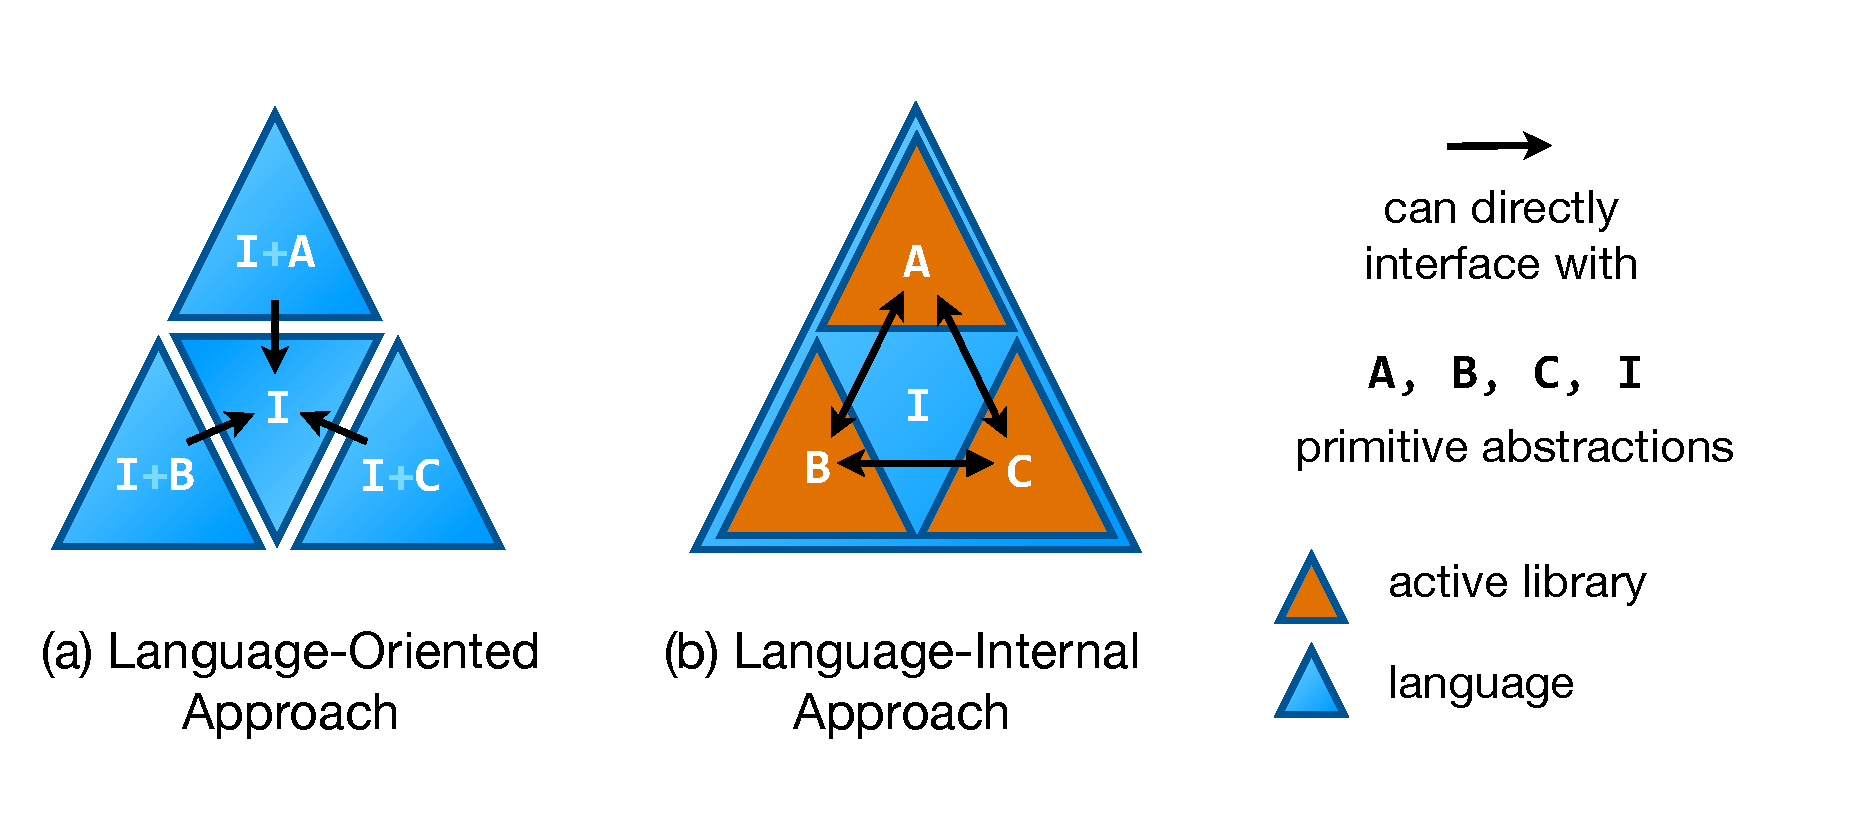
\includegraphics[scale=0.415]{approaches.pdf}
\vspace{-30px}
\caption{(a) With the language-oriented approach, different primitive abstractions are packaged into separate languages that extend and target a common intermediate language (e.g. JVM bytecode). Users can only interface with libraries written in another language via the constructs in the common language, causing \emph{interoperability problems}. (b) With the language-internal approach, the semantics of new abstractions (i.e. the logic that governs typechecking and translation to a fixed {internal language}, here labeled \texttt{I}) can be implemented directly within so-called \emph{active libraries}. Clients can import and use these abstractions directly whenever needed.}
\vspace{-10px}
\label{approaches}
\end{figure}

%As a result, domain-specific languages and new general-purpose abstractions alike have experienced relatively slow adoption in practice.
%
%Porting large codebases to new languages is difficult, and the dominant programming languages innovate slowly, so programming language.
%
%More specifically, such languages are neither \emph{internally extensible} because the language itself exposes only natural numbers and functions to its users, nor are they \emph{externally extensible} because no new behaviors can be added to the language's  implementation in a separate module from the one containing the initial implementation.

%This is the essence of a monolithic language implementation: it is impossible for anyone to modularly extend languages defined in this way. 

%Programming languages are typically designed around a monolithic collection of primitive type families and operators. Consider, as a simple example, Godel's T \cite{pfpl}, a typed lambda calculus with recursion on primitive natural numbers\todo{add statics to Appendix A}. Although a language designer may casually speak of ``extending Godel's T with primitive product and sum types'', adding these type families and associated operators to this kind of language from within is impossible. That is, Godel's T is not \emph{internally extensible}.

\emph{Internally-extensible programming languages} promise to avoid these problems by providing researchers and domain experts with a mechanism for implementing the semantics of new primitive constructs directly within libraries\todo{mention active libraries}.
%Developers of libraries need only determine whether they are appropriate for their domain, without also considering whether these constructs can be exposed in terms of abstractions appropriate to client code. 
Because primitive constructs are granularly available, rather than packaged into monolithic collections, clients can simply import any necessary primitive constructs when using code that relies on them, and thus achieve full safety, ease-of-use and performance without requiring wrappers or glue code. Providers of components thus need only consider whether primitives that they use are appropriate for their domain, without also considering whether their code might be used in a context where these primitives are not available. We diagram this competing approach in Figure \ref{approaches}(b).

%Researchers and domain experts thus gain the ability to distribute new ideas for evaluation to a broader development community without requiring the approval of maintainers of mainstream languages, large-scale porting of code or explicit interoperability layers. 

For a language-internal extension mechanism to be feasible, however, it must achieve expressiveness while also ensuring that extensions cannot compromise the safety properties of the language and its tools, nor interfere with one another. That is, extensions cannot simply be permitted to add arbitrary logic to the type system or compiler, because this would make it possible to break  type safety, decidability or adequacy theorems that are critical to the operation of the language, the compiler or other extensions. We review some previous attempts at language extensibility, and highlight how they do not adequately achieve both safety and expressiveness, in Section \ref{related-work}.
%{\color{red} transition here} Correctness properties of an extension itself should be modularly verifiable, so that its users can rely on it for verifying and compiling their own code. The mechanism must also ensure that desirable metatheoretic properties and global safety guarantees of the language cannot be weakened by extensions. And with multiple independently-developed extensions used at once, the mechanism must further guarantee that they cannot interfere with one another. 

In this paper, we introduce a language-internal extensibility mechanism called \emph{active typechecking and translation} (AT\&T) that allows developers to introduce and implement the logic governing new primitive type families and operators from within libraries. 
We argue that this can be accomplished by enriching the type-level language, rather than introducing a separate metalanguage into the system. 
To make this proposal concrete, we begin by introducing a simple core calculus, called \atlam~(for the ``actively-typed lambda calculus''), in Section \ref{atlam}. 
This calculus uses type-level computation of higher kind, along with techniques borrowed from the typed compilation literature and a form of type abstraction that ensures that the implementation details of an extension are not externally visible to guarantee the safety of the language, the decidability of typechecking and compilation and composability of extensions.

In Section \ref{examples}, we show that despite these constraints, this mechanism is expressive enough to admit, within libraries, a number of general-purpose and domain specific abstractions that normally require built-in language support. Our core calculus uses a uniform abstract syntax for primitive operators to simplify our presentation and analysis, but this syntax would be too verbose to be practical. Thus, we begin this section by showing how a key design choice made in the calculus -- to associate operators with type families, forming what we call \emph{active types} -- enables a novel type-directed desugaring mechanism that permits the use of conventional concrete syntax for language extensions. 

Our choice of a simply-typed, simply-kinded calculus where expressions are given meaning by translation to a simply-typed internal language appears to occupy a ``sweet spot'' in the design space, and relates closely to how simply-typed functional languages like  ML and Haskell are specified and implemented today. In Section \ref{design}, we briefly discuss other points in the design space of actively-typed languages and describe the sorts of abstractions that the mechanism as we have introduced it is not capable of expressing, suggesting several directions for future research. We conclude with a discussion of related work in Section \ref{related-work}.
%dependently-typed and object-oriented type-level languages, as well as the constraints governing the design of the internal language.  
%We will also note how object-oriented techniques may also be suit, because of a fundamental connection to the \emph{expression problem} \cite{expression-problem}.

%specify new typechecking rules and translation logic from within libraries. The AT\&T mechanism utilizes type-level computation of higher kind and integrates typed compilation techniques into the language to provide strong safety guarantees, while remaining straightforward and expressive.

%AT\&T is general with respect to many choices about the type-level language, the typed internal language and syntax. Choices along these dimensions can affect both expressiveness and ease-of-use. We will begin in Sec. 2 by introducing a minimal system called $@\lambda$ (the ``actively-typed lambda calculus'') that distills the essence of the mechanism in a simply-typed, simply-kinded setting. This will allow us to fully and concisely formalize the language and compiler and give several key safety theorems. We will then continue in Sec. 3 by discussing variants of this mechanism based on other basic paradigms, considering dependently-typed functional languages and object-oriented languages, discussing trade-offs between expressivity and safety when doing so. We have developed a simple prototype called Ace and have used it to develop a number of full-scale language extensions as libraries. We will briefly discuss this language and these extensions in Sec. 4.

%We note at the outset that AT\&T focuses on extending the static semantics of languages with fixed, though flexible, syntax. Language-internal syntax extension mechanisms have been developed in the past (e.g. SugarJ \cite{sugarj}) but they have also suffered from safety problems because grammar composition is not always safe when done in an  unconstrained manner. Constrained approaches that provide stronger safety guarantees have recently been outlined (e.g. Wyvern \cite{globaldsl13}) but we will leave integration of syntax extensions with semantic extensions as future work.
\section{From Extensible Compilers to Extensible Languages}\label{evolution}
To understand the genesis of our internal extension mechanism, it is helpful to begin by considering why most implementations of programming languages cannot even be  externally extended. 
Let us consider, as a simple example, an implementation of G\"odel's T, a typed lambda calculus with recursion on primitive natural numbers  \cite{pfpl}\todo{put statics in Appendix?}. 
A compiler for this language written using a functional language will invariably represent the primitive type families and operators of the object language using {closed} inductive datatypes. 
For example, a simple implementation in Standard ML may be based around these datatypes:
\begin{lstlisting}
  datatype Type = Nat | Arrow of Type * Type
  datatype Exp = Var of var 
               | Lam of var * Type * Exp
               | Ap of Exp * Exp 
               | Z | S of Exp 
               | Natrec of Exp * Exp * Exp
\end{lstlisting}

The logic governing typechecking and translation to an intermediate language (which suitable for optimization by later phases of compilation) will be implemented by exhaustive case analysis over the constructors of \lstinline{Exp}.

In an object-oriented implementation of Godel's T, we might instead encode types and operators as subclasses of abstract classes \lstinline{Type} and \lstinline{Exp}. Typechecking and translation will proceed by the ubiquitous \emph{visitor pattern} \cite{visitor} by dispatching against a set of {known} subclasses of \lstinline{Exp}. 

In either case, we encounter the same basic issue: there is no way to modularly extend the representation of primitive type families and operators and implement their associated typechecking and translation logic. 
This issue is related to the widely-discussed \emph{expression problem} (we do not consider the case of adding new functions entirely here) \cite{wadler-expression}.

A number of language mechanisms have been proposed that allow new cases to be added to datatypes and the functions that operate over them in a modular manner. 
In functional languages, we might use \emph{open datatypes} \cite{open-datatypes}. For example, if we wish to extend G\"odel's T with product types, a language supporting open datatypes might allow you to add types and operators for products to the above definitions, if they have been declared open, like this: 
\begin{lstlisting}
  newcase Prod of Type * Type extends Type
  newcase Pair of Exp * Exp extends Exp    (* Intro *)
  newcase PrL of Exp extends Exp           (* Elim Left *)
  newcase PrR of Exp extends Exp           (* Elim Right *)
\end{lstlisting}

The logic for functionality like typechecking and translation might then be specified for only the new cases. For example, a function \lstinline{typeof} that assigns a type to an expression could be extended to support the \lstinline{PrL} operator like so:
\begin{lstlisting}
  typeof PrL(e) = 
    case typeof e of 
      Prod(t1, _) => t1 
    | _ => raise TypeError("<appropriate error message>")
\end{lstlisting}

If we allow users to define new modules containing definitions like these and link them into our compiler, we have succeeded in creating an externally-extensible language implementation, albeit one where safety is not guaranteed (we will return to this point shortly). We have not, however, created an extensible programming language, because other implementations of the language will not necessarily support the same mechanism. 
If our newly-introduced constructs are exposed at a library's  interface boundary, clients using different compilers face the same problems with interoperability that those using different languages face. That is, \textbf{extending a language by extending a single implementation of it is equivalent to creating a new language}. Several prominent language ecosystems today are in a state where a prominent compiler has introduced or supported the introduction of extensions that many libraries have come to rely on, including the Glasgow Haskell Compiler, SML/NJ and the GNU compilers for C and C++. We argue that this practice should be considered harmful.

A more appropriate and useful place for extensions like this is directly within libraries. To enable this, the language must include an appropriately-constrained mechanism to introduce new type families, like \lstinline{Prod}, and operators, like \lstinline{Pair}, \lstinline{PrL} and \lstinline{PrR}, and implement the associated typechecking and translation logic. When encountering these new operators in expressions, the compiler must effectively  hand control over typechecking and translation to user-defined logic. Because this mechanism is {language-internal}, all compilers must support it to satisfy the language specification, and extensions are packaged directly within  libraries.

Statically-typed languages typically make a distinction between \emph{expressions}, which describe run-time computations, and static constructs like types and datatype declarations. The design described above suggests we may now need to add another layer to our language, an {extension language}, where extensions can be declared and implemented. In fact, we will show that \textbf{the natural place for type system extensions is within the type-level language}. The intuition is that extensions to a language's static semantics will need to manipulate types as values at compile-time. Many languages already allow users to write functions over types, effectively manipulating them as values at compile-time (see Sec. \ref{related-work} for examples). The type-level language is often constrained by its own type system (where the types of type-level values are called \emph{kinds} for clarity) that prevents type-level functions from causing problems during compilation. This is precisely the structure that a distinct extension layer would have, and so we will show that it is quite naturally to unify the two in this work.

\section{\atlam}\label{atlam}
\begin{figure}[t]
\small
$$\begin{array}{rccl}	
\textbf{programs} & \rho & ::= & \pfam{\familyDf}{\progsort} \pipe \pdef{t}{\kappa}{\tau}{\progsort} \pipe e\\
\text{primitive ops}		&	\theta	&	::= &	\topsempty \pipe 
												\topp{\theta}{\tops{op}{\kappai}{i}{a}{\tau}}\\
\\
\textbf{expressions} 				&	e	&	::=	&	\evar{x} \pipe 
														\elam{\evar{x}}{\tau}{e} \pipe 
														\eop{Fam}{op}{
															\taui
														}{
  												    		\splat{e}{1}{n}
														} \\
									& 		&		& 	\\
							
\hspace{-5pt}\textbf{type-level terms} 	& \tau 	& ::= 	& 	\tvar{t} \pipe 
														\tlam{t}{\kappa}{\tau} \pipe 
														\tapp{\tau_1}{\tau_2} \pipe
														\tnil{\kappa} \pipe \tcons{\tau_1}{\tau_2} \pipe 
									                     \tfold{\tau_1}{\tau_2}{x}{y}{\tau_3}
														\\
												
\text{type-level data}	 			& 		& \pipe	& 	 \iintlit \pipe \iop{\tau_1}{\tau_2} \pipe \tstr{str} \pipe \tunit \pipe 
														\tpair{\tau_{1}}{\tau_{2}} \pipe 
														\tfst{\tau} \pipe 
														\tsnd{\tau} 
														\\
\text{structural equality}  & & \pipe & 					\tifeq{\tau_{1}}{\tau_{2}}{\kappa}{\tau_{3}}{\tau_{4}} 
														\\														

\text{types} 						& 		& \pipe	& 	\ttypestd \pipe \tfamcase{\tau}{Fam}{x}{\tau_1}{\tau_2}\\
						%				& & \pipe & \tfamcase{\tau}{Fam}{x}{\tau_1}{\tau_2}\\
																								
\text{denotations} 				& 		 & 	\pipe	&	\tden{\tau_2}{\tau_1} \pipe \terr \pipe \tdencase{\tau}{y}{x}{\tau_1}{\tau_2}\\
 %& & \pipe & 
%														\tdencase{\tau}{y}{x}{\tau_1}{\tau_2}
%														 \\

\text{quoted IL}		&		&	\pipe	&	\titerm{\gamma} \pipe \titype{\sigma} \\

												\\
\textbf{kinds} 					& \kappa	&	::=	&	\karrow{\kappa_1}{\kappa_2} \pipe \klist{\kappa} \pipe \dint \pipe
											    \kstr \pipe
												\kunit \pipe 
												\kpair{\kappa_{1}}{\kappa_{2}} \pipe 
												\kTypeBlur \pipe \kDen \pipe 
												\kIType \pipe \kITerm
												\\
\\												
%\textbf{ops signature}			& \Theta	&	::=	&	\kOpEmpty \pipe \kOp{\Theta}{op}{\kappai}\\
%											 							&		&		&	\\
\textbf{internal terms} 				& 	\gamma	&	::=	&	\evar{x} \pipe 
												\ilam{\evar{x}}{\sigma}{\gamma} \pipe 
												\iapp{\gamma_{1}}{\gamma_{2}} \pipe
												\ifix{\evar{f}}{\sigma}{\gamma} \pipe
												\ipair{\gamma_{1}}{\gamma_{2}} \pipe 
												\ifst{\gamma} \pipe
												\isnd{\gamma}  
												\\
							& 		& 	\pipe	& 
												\iintlit \pipe \iop{\gamma_{1}}{\gamma_{2}} \pipe \iIfEq{\gamma_{1}}{\gamma_{2}}{\dint}{\gamma_{3}}{\gamma_{4}}  
												\\
 &  & \pipe & \tvalof{\tau_2}{\tau_1} \pipe \iup{\tau} \\
%\text{deabstracted}& \gamma & ::= & \mathcal{G}[\gamma, \sigma]\\
\textbf{internal types}			&	\sigma	&	::=	&    \darrow{\sigma_1}{\sigma_2} \pipe
												\dint \pipe
												\dpair{\sigma_1}{\sigma_2} \pipe
												\trepof{\tau} \pipe \dup{\tau}\\
\end{array}$$
\vspace{-10pt}
\caption{\small Syntax of \atlam. Variables $x$ are used in expressions and internal terms and are distinct from type-level variables, $\tvar{t}$. Names $\fvar{Fam}$ are family names (we assume that unique family names can be generated by some external mechanism) and $\opvar{op}$ are operator names. $\tstr{str}$ denotes string literals, $\iintlit$ denotes integer literals and $\oplus$ stands for binary operations over integers. %The productions related to the internal language are written using generators $\mathcal{G}$ and $\mathcal{S}$ to avoid duplicating the syntax of common terms.
\label{grammar}}
\end{figure}
We will now develop a core calculus, called @$\lambda$ for the ``actively-typed lambda calculus'', and discuss how to address safety concerns that arise when giving users this level of control over the semantics of a language and its implementation. 
\subsection{Overview}
\todo{remove $\Theta$ from family}The grammar of \atlam~is shown in Figure \ref{grammar}. The language is a simply-typed lambda calculus with simply-kinded type-level computation. Kinds, $\kappa$, classify type-level terms, $\tau$. 
Types classify expressions, $e$, and are type-level values of kind $\star$ (following System $F_{\omega}$ \cite{fomega}). The type-level language also includes other kinds of terms, such as type-level functions and other type-level data structures. We include lists (required by our mechanism) as well as type-level integers, strings and products for the sake of our examples (see Sec. \ref{termination} for design constraints in general).
%Some kinds of type-level values (including types themselves, but excluding type-level functions) can be compared for structural equality\todo{describe this later?}.

At the top level, programs, $\rho$, consist of a series of declarations followed by an expression. Declarations can be either bindings of type-level terms to type-level variables using \textsf{def} or a declaration of a new primitive type family using \textsf{family} (Sec. \ref{families}). Expressions can be either variables, lambdas, or applications of operators (Sec. \ref{operators}), and are ultimately given meaning by translation to a typed internal language. This language has been chosen, for simplicity, to be a variant of Plotkin's PCF with primitive integers and products, but in practice would include other constructs consistent with its role as a high-level intermediate language. Terms of this language are denoted $\gamma$ and types are denoted $\sigma$. Both of these productions also include additional forms containing type-level terms, $\tau$; these are used during compilation and will be explained below.

\subsection{Example: Natural Numbers}
\begin{figure}[t]
\small
%\begin{lstlisting}
%family Nat of 1 ~ _.\/(int) {
%	z(i:1, a. case len a =_Z 0 then [[Nat<()> ==> 0]] else err);
%	s(i:1, a. get_last_arg a err (\a1. 
%	  dencase a1 of [[t1 ==> v1]] => 
%	    if t1 =_* Nat<()> then [[Nat<()> ==> ^(v1) + 1]] else err
%	  ow err))
%}
%\end{lstlisting}
\begin{flalign}
&\family{Nat}{\kunit}{\\
&\quad\tops{z}{\kunit}{i}{a}{
	\tapp{\tapp{\tvar{no\_args}}{\tvar{a}}}{
		\tlam{\_}{\kunit}{\tden{\titerm{0}}{\ttype{Nat}{\tunit}}}
	}};\\
&\quad\tops{s}{\kunit}{i}{a}{
	\tapp{
		\tapp{\tvar{last\_arg}}{\tvar{a}}}{\tlam{t1}{\kTypeBlur}{\tlam{v1}{\kITerm}{
			\\
			&\quad\quad\tapp{\tapp{\tapp{\tvar{check\_type}}{\tvar{t1}}}{\ttype{Nat}{\tunit}}}{
				\tden{\titerm{\iup{\tvar{v1}}+1}}{\ttype{Nat}{\tunit}}
			}
		}}
		}
	};\\
&\quad\tops{rec}{\kunit}{i}{a}{
	\tapp{\tapp{\tvar{next\_arg}}{\tvar{a}}}{\tlam{t1}{\kTypeBlur}{\tlam{v1}{\kITerm}{\tlam{a}{\klist{\kDen}}{\\
	&\quad\quad\tapp{\tapp{\tvar{next\_arg}}{\tvar{a}}}{\tlam{t2}{\kTypeBlur}{\tlam{v2}{\kITerm}{\tlam{a}{\klist{\kDen}}{\\
	&\quad\quad \tapp{\tapp{\tvar{last\_arg}}{\tvar{a}}}{\tlam{t3}{\kTypeBlur}{\tlam{v3}{\kITerm}{\\
	&\quad\quad \tapp{\tapp{\tapp{\tvar{check\_type}}{\tvar{t1}}}{\ttype{Nat}{\tunit}}}{(\\
	&\quad\quad \tapp{\tapp{\tapp{\tvar{check\_type}}{\tvar{t3}}}{\ttype{Arrow}{(\ttype{Nat}{\tunit},\ttype{Arrow}{(\tvar{t2},\tvar{t2})})}}}{(\\
		&\quad\quad c
	)}}
	}}}}}}}}}}}}
\\
&}{XXX}{i}{\titype{\dint}}
\end{flalign}
\caption{Example: primitive natural numbers and $n$-ary ($n > 1$) products in \atlam.}
\label{example}
\end{figure}
To make our discussion of each of these components of the calculus concrete, we will begin with an example showing how to introduce primitive natural numbers, implemented as integers internally, as a user-defined extension. 

\subsection{Central Compilation Judgement}
\begin{figure}[t]
\small
\begin{mathpar}
\inferrule{
	\overbrace{\progOK{\emptyctx}{\fvarCtx_0}{\rho}}^{\text{\normalsize Kind Checking}}\\
	\overbrace{\pcompiles{\fvalCtx_0}{\rho}{\gamma}}^{\text{\normalsize Active Typechecking and Translation}}
}{
	\ptcc{\rho}{\gamma}
}
\end{mathpar}
\vspace{-10pt}
\caption{\small Central Compilation Judgement of \atlam.}
\label{ccj}
\end{figure}
The \emph{central compilation judgement}, shown in Figure \ref{ccj}, captures the two phases of compilation: kind checking and active typechecking and translation. The latter phase requires normalizing type-level terms to type-level values, so the  kind checking phase preceding it will ensure that this process not ``get stuck'', as we will elaborate upon when discussing safety and decidability in Sec. \ref{safety}.

\subsection{Indexed Type Families and Types}\label{families}
Declaring a new primitive indexed type family by using \textsf{family} can be compared to adding a new constructor to the compiler's \lstinline{Type} datatype, as suggested in Section \ref{evolution}. The kind of type-level data that the family is indexed by is specified by $\kappaidx$. For example, a base type like $\tvar{nat}$ can be thought of as being the only type in a family, $\fvar{Nat}$, trivially indexed by the unit value, of kind $\kunit$, while families like $\fvar{Pair}$ might be indexed by a pair of types, of kind $\kpair{\kTypeBlur}{\kTypeBlur}$. A type (that is, a type-level term of kind $\kTypeBlur$) is created by naming a family that has been previously been introduced and providing an index of the appropriate kind. For example, $\ttype{Prod}{\tpair{\tvar{nat}}{\tvar{nat}}}$ is the type of a pair of natural numbers in a context where the families $\fvar{Prod}$ and $\fvar{Nat}$ have been introduced as described above and the type-level variable $\tvar{nat}$ has been bound to the type $\ttype{Nat}{\tunit}$.

\subsection{Indexed Operator Families and Active Types}\label{operators}
We build in lambdas as the only binding structure in the language to simplify the core calculus. All other operators are associated with a type. For example, nat / tuples / records.

Operator families. 

\subsection{Active Typechecking and Translation}

\subsection{Abstract Representations}

\begin{figure}[t]
\small
$\fbox{\inferrule{}{\progOKX{\progsort}}}$
~~~$\tvarCtx ::= \emptyctx \pipe \tvarCtxX{t}{\kappa}$~~~
$\fCtx ::= \Sigma_0	 \pipe \fvarCtxX$
\begin{mathpar}
\inferrule[family decl kinding]{
	\fvar{Fam} \notin \fvarCtx\\
	\kEq{\kappaidx}\\
	\opType{\tvarCtx}{\fvarCtxX}{\theta}{\Theta}\\\\
	\tKind{\tvarCtx, \tvar{i}:{\kappaidx}}{\fvarCtxX}{\tau}{\kIType}\\
	\progOK{\tvarCtx}{\fvarCtxX}{\rho}
}{
	\progOKX{\pfam{\familyDf}{\rho}}
}

\inferrule[type-level bind kinding]{
	\tKindX{\tau}{\kappa}\\
	\progOK{\tvarCtxX{t}{\kappa}}{\fvarCtx}{\rho}
}{
	\progOKX{\pdef{t}{\kappa}{\tau}{\rho}}
}

\inferrule[exp kinding]{
	\exprOK{\tvarCtx}{\emptyctx}{\fvarCtx}{e}
}{
	\progOKX{e}
}
\end{mathpar}
$\fbox{$\tKindX{\theta}{\Theta}$}$
\begin{mathpar}
\inferrule[no ops]{ }{
	\tKindX{\topsempty}{\kOpEmpty}
}

\inferrule[ops]{
	\opType{\tvarCtx}{\fvarCtx}{\theta}{\Theta}\\
	\opvar{op} \notin \theta\\
	\tKind{\tvarCtx, \tOfKind{\tvar{i}}{\kappai}, \tOfKind{\tvar{a}}{\klist{\kDen}}}{\fvarCtx}{\tau}{\kDen}
}{
	\opType{\tvarCtx}{\fvarCtx}{\topp{\theta}{\tops{op}{\kappai}{i}{a}{\tau}}}{
	\kOp{\Theta}{op}{\kappai}}
}
\end{mathpar}
$\fbox{$\exprOKX{e}$}$
~~~$\itvarCtx ::= \emptyctx \pipe \itvarCtx, \evar{x}$
\begin{mathpar}
\inferrule[e-var-kind]{ }{
	\exprOK{\tvarCtx}{\itvarCtx, \evar{x}}{\fvarCtx}{\evar{x}}
}

\inferrule[e-lam-kind]{
	\tKindX{\tau}{\kTypeBlur}\\
	\exprOK{\tvarCtx}{\eivarCtxX{x}}{\fvarCtx}{e}
}{
	\exprOKX{\elam{\evar{x}}{\tau}{e}}
}

\inferrule[e-op-kind]{
	\fvarOfType{Fam}{\kappaidx}{\Theta} \in \fvarCtx\\
	\kOpS{op}{\kappai} \in \Theta\\
	\tKindX{\taui}{\kappai}\\\\
	\exprOKX{e_1}\\
	\cdots\\
	\exprOKX{e_n}
}{
	\exprOKX{\eop{Fam}{op}{\taui}{\splat{e}{1}{n}}}
}
\end{mathpar}
\caption{\small Kinding for programs. Variable contexts $\tvarCtx$ and $\itvarCtx$ obey standard structural properties. Kinding for type-level terms in Figure \ref{kindtl}. \ \label{kindprof}}
\end{figure}
\begin{figure}[t]
\small
$\fbox{\inferrule{}{\pcompilesX{\rho}}}$
~~~$\fvalCtx ::= \fvalCtx_0 \pipe \fvalCtxX{\fvalDf}$
\begin{mathpar}
\inferrule[att-fam]{
	\pcompiles{\fvalCtxX{\fvalDf}}{\rho}{\gamma}
}{
	\pcompilesX{\pfam{\familyDf}{\rho}}
}

\inferrule[att-def]{
	\tEvalX{\tau}{\tau'}\\
	\pcompilesX{\subst{\tau'}{\tvar{t}}{\rho}}
}{
	\pcompilesX{\pdef{t}{\kappa}{\tau}{\rho}}
}

\inferrule[att-exp]{
	\ecompiles{\emptyctx}{\fvalCtx}{e}{\tau}{\ghat}\\
	\eraseX{\ghat}{\gamma}
}{
	\pcompilesX{e}
}
\end{mathpar}
$\fbox{\inferrule{}{\ecompilesX{e}{\tau}{\ghat}}}$
~~~$\etCtx ::= \emptyctx \pipe \etCtxX{x}{\tau}$
\begin{mathpar}
\inferrule[att-var]{ }{
	\ecompiles{\etCtxX{x}{\tau}}{\fvalCtx}{\evar{x}}{\tau}{\evar{x}}
}

\inferrule[att-lam]{
	\tEvalX{\tau_1}{\ttype{Fam}{\tauidx}}\\
	\ecompiles{\etCtxX{x}{\ttype{Fam}{\tauidx}}}{\fvalCtx}{e}{\tau_2}{\ghat}\\\\
	\tauisdel{Arrow}{\fvalCtx}{Fam}{\tauidx}{\dbar}\\
}{
	\ecompiles{\etCtx}{\fvalCtx}{\elam{\evar{x}}{\tau_1}{e}}{\ttype{Arrow}{\tpair{\ttype{Fam}{\tauidx}}{\tau_2}}}{\ilam{\evar{x}}{\dbar}{\ghat}}
}

\inferrule[att-op]{
	\fvalDf \in \fvalCtx\\
	\tops{op}{\kappai}{i}{a}{\tauop} \in \theta\\
	\tEvalX{\taui}{\taui'}\\\\
	\ecompiles{\etCtx}{\fvalCtx}{e_1}{\tau_1}{\ghat_1}~~~~
	\cdots~~~~
	\ecompiles{\etCtx}{\fvalCtx}{e_n}{\tau_n}{\ghat_n}\\
	\text{$\begin{array}{c}
		\left[\text{$\begin{array}{r}
			\taui'/\tvar{i}\\
			\tden{\titerm{\ghat_1}}{\tau_1} :: \cdots :: \tden{\titerm{\ghat_n}}{\tau_n} :: \tnil{\kDen}/\tvar{a}
			\end{array}$}\right]\tauop
		\Downarrow
		\tden{\titerm{\ghat}}{\ttype{Fam'}{\tauidx}}
		\end{array}$}\\
	\tauisdel{Fam}{\fvalCtx}{Fam'}{\tauidx}{\dbar}\\
	\eCtxTogCtx{Fam}{\fvalCtx}{\etCtx}{\gtCtx}\\
	\checkRC{\gtCtx}{Fam}{\fvalCtx}{\ghat}{\dbar}
}{
	\ecompiles{\etCtx}{\fvalCtx}{\eop{Fam}{op}{\taui}{\splat{e}{1}{n}}}{\ttype{Fam'}{\tauidx}}{\ghat}
}
\end{mathpar}
\caption{\small Active typechecking and translation}
\end{figure}
\begin{figure}[t]
\small
\vspace{-15pt}
$\fbox{\inferrule{}{\tKindX{\tau}{\kappa}}}$
\begin{mathpar}
\small
\inferrule[var kind]{
}{
  \tKind{\tvarCtxX{t}{\kappa}}{\fvarCtx}{\tvar{t}}{\kappa}
}

\inferrule[k-arrow intro]{
  \tKind{\tvarCtxX{t}{\kappa_1}}{\fvarCtx}{\tau}{\kappa_2}
}{
  \tKindX{\tlam{t}{\kappa_1}{\tau}}{\karrow{\kappa_1}{\kappa_2}}
}

\inferrule[k-arrow elim]{
  \tKindX{\tau_1}{\karrow{\kappa_1}{\kappa_2}}\\
  \tKindX{\tau_2}{\kappa_1}
}{
  \tKindX{\tapp{\tau_1}{\tau_2}}{\kappa_2}
}
\\
\text{\color{gray} (standard statics for integers, strings, products and lists omitted)}
\\
%%
%%\inferrule{ }{
%%	\tKindX{\tstr{str}}{\kstr}
%%}(\text{str}^I_\tau)
%%
%%\inferrule{ }{
%%	\tKindX{\tunit}{\kunit}
%%}(\text{1}^I_\tau)
%%
%%\inferrule{
%%	\tKindX{\tau_1}{\kappa_1}\\
%%	\tKindX{\tau_2}{\kappa_2}
%%}{
%%	\tKindX{\tpair{\tau_1}{\tau_2}}{\kpair{\kappa_1}{\kappa_2}}
%%}({\times}^I_\tau)
%%
%%\inferrule{
%%	\tKindX{\tau}{\kpair}{\kappa_1}{\kappa_2}
%%}{
%%	\tKindX{\tfst{\tau}}{\kappa_1}
%%}({\times}^{E1}_\tau)
%%
%%\inferrule{
%%	\tKindX{\tau}{\kpair}{\kappa_1}{\kappa_2}
%%}{
%%	\tKindX{\tsnd{\tau}}{\kappa_2}
%%}({\times}^{E2}_\tau)
%%\inferrule{ }{
%%\inferrule{
%%	\tKindX{\tau_{1}}{\kappa_{1}}\\
%%	\tKindX{\tau_{2}}{\kappa_{2}}
%%}{
%%	\tKindX{\tpair{\tau_{1}}{\tau_{2}}}{\kpair{\kappa_{1}}{\kappa_{2}}}
%%}~(\times_\tau)
%%
%%\inferrule{
%%	\tKindX{\tau}{\kpair{\kappa_{1}}{\kappa_{2}}}
%%}{
%%	\tKindX{\tfst{\tau}}{\kappa_{1}}
%%}~(\text{fst}_\tau)
%%
%%\inferrule{
%%	\tKindX{\tau}{\kpair{\kappa_{1}}{\kappa_{2}}}
%%}{
%%	\tKindX{\tsnd{\tau}}{\kappa_{2}}
%%}~(\text{snd}_\tau)
%%
%% TODO: list
\inferrule[eq kind]{
	\kEq{\kappa}\\
	\tKindX{\tau_1}{\kappa}\\
	\tKindX{\tau_2}{\kappa}\\\\
	\tKindX{\tau_3}{\kappa'}\\
	\tKindX{\tau_4}{\kappa'}
}{
	\tKindX{\tifeq{\tau_1}{\tau_2}{\kappa}{\tau_3}{\tau_4}}{\kappa'}
}

\inferrule[type intro]{
	\fvarOfTypeDf \in \fvarCtx\\\\
	\tKind{\tvarCtx}{\fvarCtx}{\tauidx}{\kappaidx}
}{
	\tKindX{\ttype{Fam}{\tauidx}}{\kTypeBlur}
}

\inferrule[type elim]{
	\fvarOfTypeDf \in \fvarCtx\\
	\tKindX{\tau}{\kTypeBlur}\\\\
	\tKind{\tvarCtxX{x}{\kappaidx}}{\fvarCtx}{\tau_0}{\kappa}\\
	\tKindX{\tau_1}{\kappa}
}{
	\tKind{\tvarCtx}{\fvarCtx}{\tfamcase{\tau}{Fam}{x}{\tau_0}{\tau_1}}{\kappa}
}

\inferrule[den intro valid]{
	\tKindX{\tautype}{\kTypeBlur}\\\\
	\tKindX{\tauval}{\kITerm}
}{
	\tKindX{\tden{\tauval}{\tautype}}{\kDen}
}

\inferrule[den intro err]{ }{
	\tKindX{\terr}{\kDen}
}

\inferrule[den elim]{
	\tKindX{\tauden}{\kDen}\\
	\tKind{\tvarCtx, \tOfKind{\tvar{x}}{\kITerm}, \tOfKind{\tvar{y}}{\kTypeBlur}}{\fvarCtx}{\tau_1}{\kappa}\\
	\tKindX{\tau_2}{\kappa}
}{
	\tKindX{\tdencase{\tauden}{y}{x}{\tau_1}{\tau_2}}{\kappa}
}

\inferrule[iterm intro]{
	\isIterm{\tvarCtx}{\emptyctx}{\fvarCtx}{\ghat}
}{
	\tKindX{\titerm{\ghat}}{\kITerm}
}

\inferrule[itype intro]{
	\isItype{\tvarCtx}{\fvarCtx}{\dhat}
}{
	\tKindX{\titype{\dhat}}{\kIType}
}
\end{mathpar}
$\fbox{$\kEq{\kappa}$}$
\begin{mathpar}
\inferrule[t-eq]{ }{
	\kEq{\kTypeBlur}
}

\inferrule[z-eq]{ }{
	\kEq{\dint}
}

\inferrule[str-eq]{ }{
	\kEq{\kstr}
}

\inferrule[u-eq]{ }{
	\kEq{\kunit}
}

\inferrule[prod-eq]{
	\kEq{\kappa_1}\\
	\kEq{\kappa_2}
}{
	\kEq{\kpair{\kappa_1}{\kappa_2}}
}

\inferrule[list-eq]{
	\kEq{\kappa}
}{
	\kEq{\klist{\kappa}}
}
\end{mathpar}
$\fbox{$\isItermX{\ghat}$}$
\begin{mathpar}
\inferrule[i-var kind]{ }{
	\isIterm{\tvarCtx}{\eivarCtxX{x}}{\fvarCtx}{\evar{x}}
}

\inferrule[i-lam kind]{
	\isItypeX{\dhat}\\\\
	\isIterm{\tvarCtx}{\eivarCtxX{x}}{\fvarCtx}{\ghat}
}{
	\isItermX{\ilam{\evar{x}}{\dhat}{\ghat}}
}

\inferrule[i-fix kind]{
	\isItypeX{\dhat}\\\\
	\isIterm{\tvarCtx}{\eivarCtxX{x}}{\fvarCtx}{\ghat}
}{
	\isItermX{\ifix{\evar{f}}{\dhat}{\ghat}}
}
\\
\text{\color{gray} (omitted forms have trivially recursive rules)}\\\vspace{-3pt}
\\
\inferrule[iterm unquote kind]{
	\tKindX{\tau}{\kITerm}
}{
	\isItermX{\iup{\tau}}
}

\inferrule[val from den kind]{
	\tKindX{\tautype}{\kTypeBlur}\\
	\tKindX{\tauval}{\kITerm}
}{
	\isItermX{\tvalof{\tauval}{\tautype}}
}
\end{mathpar}
$\fbox{$\isItypeX{\dhat}$}$
\begin{mathpar}
\inferrule[i-int kind]{ }{
	\isItypeX{\dint}
}

\inferrule[i-prod kind]{
	\isItypeX{\dhat_1}\\\\
	\isItypeX{\dhat_2}
}{
	\isItypeX{\dpair{\dhat_1}{\dhat_2}}
}

\inferrule[i-arrow kind]{
	\isItypeX{\dhat_1}\\\\
	\isItypeX{\dhat_2}
}{
	\isItypeX{\darrow{\dhat_1}{\dhat_2}}
}

\inferrule[itype unquote kind]{
	\tKindX{\tau}{\kIType}
}{
	\isItypeX{\dup{\tau}}
}

\inferrule[rep from type kind]{
	\tKindX{\tau}{\kTypeBlur}
}{
	\isItypeX{\trepof{\tau}}
}
\end{mathpar}
\caption{\small Kinding for type-level terms}
\end{figure}

\begin{figure}
\small
$\fbox{$\tEvalX{\tau}{\tau'}$}$
\begin{mathpar}
\inferrule[tl-lam eval]{ }{
	\tEvalX{\tlam{t}{\kappa}{\tau}}{\tlam{t}{\kappa}{\tau}}
}

\inferrule[tl-ap eval]{
	\tEvalX{\tau_1}{\tlam{t}{\kappa}{\tau}}\\
	\tEvalX{\tau_2}{\tau_2'}\\
	\tEvalX{\subst{\tau_2'}{\tvar{t}}{\tau}}{\tau'}
}{
	\tEvalX{\tapp{\tau_1}{\tau_2}}{\tau'}
}

\text{\color{gray} (standard evaluation rules for integers, strings, products and lists omitted)}

\inferrule[tl-eq eval eq]{
	\tEvalX{\tau_1}{\tau_1'}\\
	\tEvalX{\tau_2}{\tau_1'}\\
	\tEvalX{\tau_3}{\tau_3'}
}{
	\tEvalX{\tifeq{\tau_1}{\tau_2}{\kappa}{\tau_3}{\tau_4}}{\tau_3'}
}

\inferrule[tl-eq eval neq]{
	\tEvalX{\tau_1}{\tau_1'}\\
	\tEvalX{\tau_2}{\tau_2'}\\
	\tau_1' \neq \tau_2'\\
	\tEvalX{\tau_4}{\tau_4'}
}{
	\tEvalX{\tifeq{\tau_1}{\tau_2}{\kappa}{\tau_3}{\tau_4}}{\tau_4'}
}

\inferrule[type eval]{
	\tEvalX{\tauidx}{\tauidx'}
}{
	\tEvalX{\ttype{Fam}{\tauidx}}{\ttype{Fam}{\tauidx'}}
}

\inferrule[famcase eval match]{
	\tEvalX{\tau}{\ttype{Fam}{\tauidx}}\\
	\tEvalX{\subst{\tauidx}{\tvar{x}}{\tau_1}}{\tau_1'}
}{
	\tEvalX{\tfamcase{\tau}{Fam}{x}{\tau_1}{\tau_2}}{\tau_1'}
}

\inferrule[famcase eval fail]{
	\tEvalX{\tau}{\ttype{Fam'}{\tauidx}}\\
	\fvar{Fam} \neq \fvar{Fam'}\\
	\tEvalX{\tau_2}{\tau_2'}
}{
	\tEvalX{\tfamcase{\tau}{Fam}{x}{\tau_1}{\tau_2}}{\tau_2'}
}

\inferrule[den eval]{
	\tEvalX{\tautype}{\tautype'}\\
	\tEvalX{\tauval}{\tauval'}
}{
	\tEvalX{\tden{\tauval}{\tautype}}{\tden{\tauval'}{\tautype'}}
}

\inferrule[err eval]{ }{
	\tEvalX{\terr}{\terr}
}

\inferrule[dencase eval valid]{
	\tEvalX{\tauden}{\tden{\tauval}{\tautype}}\\
	\tEvalX{[\tautype/\tvar{x}, \titerm{\tvalof{\tauval}{\tautype}}/\tvar{y}]\tau_1}{\tau_1'}
}{
	\tEvalX{\tdencase{\tauden}{y}{x}{\tau_1}{\tau_2}}{\tau_1'}
}

\inferrule[dencase eval err]{
	\tEvalX{\tauden}{\terr}\\
	\tEvalX{\tau_2}{\tau_2'}
}{
	\tEvalX{\tdencase{\tauden}{y}{x}{\tau_1}{\tau_2}}{\tau_2'}
}

\inferrule[iterm quote eval]{
	\tiEvalX{\ghat}{\ghat'}
}{
	\tEvalX{\titerm{\ghat}}{\titerm{\ghat'}}
}

\inferrule[itype quote eval]{
	\tiEvalX{\dhat}{\dhat'}
}{
	\tEvalX{\titype{\dhat}}{\titype{\dhat'}}
}
\end{mathpar}
$\fbox{$\tiEvalX{\ghat}{\ghat'}$}$
\begin{mathpar}
\inferrule[i-var eval]{ }{
	\tiEvalX{\evar{x}}{\evar{x}}
}

\inferrule[i-lam eval]{
	\tiEvalX{\dhat}{\dhat'}\\
	\tiEvalX{\ghat}{\ghat'}
}{
	\tiEvalX{\ilam{\evar{x}}{\dhat}{\ghat}}{\ilam{\evar{x}}{\dhat'}{\ghat'}}
}

\inferrule[i-fix eval]{
	\tiEvalX{\dhat}{\dhat'}\\
	\tiEvalX{\ghat}{\ghat'}
}{
	\tiEvalX{\ifix{\evar{f}}{\dhat}{\ghat}}{\ifix{\evar{f}}{\dhat'}{\ghat'}}
}
\\
\text{\color{gray} (omitted forms have trivially recursive rules)}
\\
\inferrule[iterm unquote eval]{
	\tEvalX{\tau}{\tau'}
}{
	\tiEvalX{\iup{\tau}}{\iup{\tau'}}
}

\inferrule[val from den eval]{
	\tEvalX{\tautype}{\tautype'}\\
	\tEvalX{\tauval}{\tauval'}
}{
	\tiEvalX{\tvalof{\tauval}{\tautype}}{\tvalof{\tauval'}{\tautype'}}
}
\end{mathpar}
$\fbox{$\tiEvalX{\sigma}{\sigma'}$}$
\begin{mathpar}
\inferrule[i-int eval]{ }{
	\tiEvalX{\dint}{\dint}
}

\inferrule[i-prod eval]{
	\tiEvalX{\dhat_1}{\dhat_1'}\\
	\tiEvalX{\dhat_2}{\dhat_2'}
}{
	\tiEvalX{\dpair{\dhat_1}{\dhat_2}}{\dpair{\dhat_1'}{\dhat_2'}}
}

\inferrule[i-arrow eval]{
	\tiEvalX{\dhat_1}{\dhat_1'}\\
	\tiEvalX{\dhat_2}{\dhat_2'}
}{
	\tiEvalX{\darrow{\dhat_1}{\dhat_2}}{\darrow{\dhat_1'}{\dhat_2'}}
}

\inferrule[itype unquote eval]{
	\tEvalX{\tau}{\tau'}
}{
	\tiEvalX{\dup{\tau}}{\dup{\tau'}}
}

\inferrule[rep from type eval]{
	\tEvalX{\tau}{\tau'}
}{
	\tiEvalX{\trepof{\tau}}{\trepof{\tau'}}
}
\end{mathpar}
\caption{\small Evaluation semantics for type-level terms}
\end{figure}

\begin{figure}
\small
$\fbox{\inferrule{}{\delfromtau{Fam}{\fvalCtx}{\tau}{\dbar}}}$
~~~$\fvalCtx ::= \fvalCtx_0 \pipe \fvalCtx, \fvalDf$
\begin{mathpar}
\inferrule[abs rep from type]{
	\fval{Fam'}{\theta}{i}{\tau} \in \fvalCtx\\
	\tEvalX{[\tauidx/\tvar{i}]\tau}{\titype{\dhat}}\\
	\ddbarX{\dhat}{\dbar}
}{
	\tauisdel{Fam}{\fvalCtx}{Fam'}{\tauidx}{\dbar}
}
\end{mathpar}
$\fbox{\inferrule{}{\ddbarX{\dhat}{\dbar}}}$
\begin{mathpar}
\inferrule[abs int]{ }{
	\ddbarX{\dint}{\dint}
}

\inferrule[abs arrow]{
	\ddbarX{\dhat_1}{\dbar_1}\\
	\ddbarX{\dhat_2}{\dbar_2}
}{
	\ddbarX{\darrow{\dhat_1}{\dhat_2}}{\darrow{\dbar_1}{\dbar_2}}
}

\inferrule[abs prod]{
	\ddbarX{\dhat_1}{\dbar_1}\\
	\ddbarX{\dhat_2}{\dbar_2}
}{
	\ddbarX{\dpair{\dhat_1}{\dhat_2}}{\dpair{\dbar_1}{\dbar_2}}
}

\inferrule[abs+cancel unquote]{
	\ddbarX{\dhat}{\dbar}
}{
	\ddbarX{\dup{\titype{\dhat}}}{\dbar}
}

\inferrule[abs rep from type visible]{
	\fvalDf \in \fvalCtx\\
	\tEvalX{[\tauidx/\tvar{i}]\tau}{\titype{\dhat}}\\
	\ddbarX{\dhat}{\dbar}
}{
	\ddbarX{\trepof{\ttype{Fam}{\tauidx}}}{\dbar}
}

\inferrule[abs rep from type hidden]{
	\fvar{Fam} \neq \fvar{Fam'}
}{
	\ddbarX{\trepof{\ttype{Fam'}{\tauidx}}}{\trepof{\ttype{Fam'}{\tauidx}}}
}
\end{mathpar}
$\fbox{\inferrule{}{\eCtxTogCtxX{\etCtx}{\gtCtx}}}$
~~~$\gtCtx ::= \emptyctx \pipe \gtCtxX{x}{\dbar}$
\begin{mathpar}
\inferrule[abs empty]{ }{
	\eCtxTogCtxX{\emptyctx}{\emptyctx}
}

\inferrule[abs ctx]{
	\eCtxTogCtxX{\etCtx}{\gtCtx}\\
	\delfromtau{Fam}{\fvalCtx}{\tau}{\dbar}
}{
	\eCtxTogCtxX{\etCtxX{x}{\tau}}{\gtCtxX{x}{\dbar}}
}
\end{mathpar}
$\fbox{\inferrule{}{\checkRCX{\ghat}{\dbar}}}$
\begin{mathpar}
\inferrule[abs i-var]{ }{
	\checkRC{\gtCtxX{x}{\dbar}}{Fam}{\fvalCtx}{\evar{x}}{\dbar}
}

\inferrule[abs i-lam]{
	\ddbarX{\dhat_1}{\dbar_1}\\
	\checkRC{\gtCtxX{x}{\dbar_1}}{Fam}{\fvalCtx}{\gamma}{\dbar_2}
}{
	\checkRCX{\ilam{x}{\dhat_1}{\gamma}}{\darrow{\dbar_1}{\dbar_2}}
}

\inferrule[abs i-ap]{
	\checkRCX{\ghat_1}{\darrow{\dbar_1}{\dbar_2}}\\\\
	\checkRCX{\ghat_2}{\dbar_1}
}{
	\checkRCX{\iapp{\ghat_1}{\ghat_2}}{\dbar_2}
}

\inferrule[abs i-fix]{
	\ddbarX{\dhat}{\dbar}\\
	\checkRC{\gtCtxX{x}{\dbar}}{Fam}{\fvalCtx}{\ghat}{\dbar}
}{
	\checkRCX{\ifix{x}{\dhat}{\ghat}}{\dbar}
}
\\
\text{\color{gray} (standard statics for integers and products omitted)}
\\
%\inferrule[abs int]{ }{
%	\checkRCX{\iintlit}{\dint}
%}
%
%\inferrule[abs op]{
%	\checkRCX{\gamma_1}{\dint}\\
%	\checkRCX{\gamma_2}{\dint}
%}{
%	\checkRCX{\iop{\gamma_1}{\gamma_2}}{\dint}
%}
%
%\inferrule[abs pair]{
%	\checkRCX{\gamma_1}{\dbar_1}\\
%	\checkRCX{\gamma_2}{\dbar_2}
%}{
%	\checkRCX{\ipair{\gamma_1}{\gamma_2}}{\dpair{\dbar_1}{\dbar_2}}
%}
%
%\inferrule[abs fst]{
%	\checkRCX{\gamma}{\dpair{\dbar_1}{\dbar_2}}
%}{
%	\checkRCX{\ifst{\gamma}}{\dbar_1}
%}
%
%\inferrule[abs snd]{
%	\checkRCX{\gamma}{\dpair{\dbar_1}{\dbar_2}}
%}{
%	\checkRCX{\isnd{\gamma}}{\dbar_2}
%}
%
\inferrule[abs if eq]{
	\checkRCX{\ghat_1}{\dint}\\
	\checkRCX{\ghat_2}{\dint}\\\\
	\checkRCX{\ghat_3}{\dbar}\\
	\checkRCX{\ghat_4}{\dbar}
}{
	\checkRCX{\iIfEq{\ghat_1}{\ghat_2}{\dint}{\ghat_3}{\ghat_4}}{\dbar}
}

\inferrule[abs iterm unquote]{
	\checkRCX{\ghat}{\dbar}
}{
	\checkRCX{\iup{\titerm{\ghat}}}{\dbar}
}

\inferrule[abs val from den visible]{
	\tauisdel{Fam}{\fvalCtx}{Fam}{\tauidx}{\dbar}\\
	\checkRCX{\ghat}{\dbar}
}{
	\checkRCX{\tvalof{\titerm{\ghat}}{\ttype{Fam}{\tauidx}}}{\dbar}
}

\inferrule[abs val from den hidden]{
	\fvar{Fam} \neq \fvar{Fam'}\\
	\tauisdel{Fam}{\fvalCtx}{Fam'}{\tauidx}{\dbar}\\
	\checkRCX{\ghat}{\dbar}
}{
	\checkRCX{\tvalof{\titerm{\ghat}}{\ttype{Fam'}{\tauidx}}}{\trepof{\ttype{Fam'}{\tauidx}}}
}
\end{mathpar}
\caption{\small Abstracted internal typing}
\end{figure}
\begin{figure}[t]
\small
$\fbox{\inferrule{}{\eraseX{\dbar}{\sigma}}}$
\begin{mathpar}
\inferrule[deabs int]{ }{
	\eraseX{\dint}{\dint}
}

\inferrule[deabs arrow]{
	\eraseX{\dbar_1}{\sigma_1}\\\\
	\eraseX{\dbar_2}{\sigma_2}
}{
	\eraseX{\darrow{\dbar_1}{\dbar_2}}{\darrow{\sigma_1}{\sigma_2}}
}

\inferrule[deabs prod]{
	\eraseX{\dbar_1}{\sigma_1}\\\\
	\eraseX{\dbar_2}{\sigma_2}
}{
	\eraseX{\dpair{\dbar_1}{\dbar_2}}{\dpair{\sigma_1}{\sigma_2}}
}

\inferrule[deabs  rep from type hidden]{
	\fvalDf \in \fvalCtx\\
	\tEvalX{[\tauidx/\tvar{i}]\tau}{\titype{\dhat}}\\\\
	\ddbarX{\dhat}{\dbar}\\
	\eraseX{\dbar}{\sigma}
}{
	\eraseX{\trepof{\ttype{Fam}{\tauidx}}}{\sigma}
}
\end{mathpar}
$\fbox{\inferrule{}{\eraseX{\ghat}{\gamma}}}$
\begin{mathpar}
\inferrule[deabs i-var]{ }{
	\eraseX{\evar{x}}{\evar{x}}
}

\inferrule[deabs i-lam]{
	\ddbar{\_}{\fvalCtx}{\dhat}{\dbar}\\
	\eraseX{\dbar}{\sigma}\\
	\eraseX{\ghat}{\gamma}
}{
	\eraseX{\ilam{x}{\dhat}{\ghat}}{\ilam{x}{\sigma}{\gamma}}
}

%\inferrule[deabs ap]{
%	\eraseX{\ghat_1}{\ghat_1}\\
%	\eraseX{\ghat_2}{\ghat_2}
%}{
%	\eraseX{\iapp{\ghat_1}{\ghat_2}}{\iapp{\ghat_1}{\ghat_2}}
%}
%
\inferrule[deabs i-fix]{
	\ddbar{\_}{\fvalCtx}{\dhat}{\dbar}\\
	\eraseX{\dbar}{\sigma}\\
	\eraseX{\ghat}{\gamma}
}{
	\eraseX{\ifix{x}{\dhat}{\ghat}}{\ifix{x}{\sigma}{\gamma}}
}
\\
\text{\color{gray} (omitted forms have trivially recursive rules)}
\\
\inferrule[deabs unquote]{
	\eraseX{\ghat}{\gamma}
}{
	\eraseX{\iup{\titerm{\ghat}}}{\gamma}
}

\inferrule[deabs val from den hidden]{
	\eraseX{\ghat}{\gamma}
}{
	\eraseX{\tvalof{\titerm{\ghat}}{\ttype{Fam}{\tauidx}}}{\gamma}
}
\end{mathpar}
\caption{\small Deabstraction rules}
\end{figure}
%
%family RECORD of (string, type) dict {
%  new(idx, args. foldl (fn (x, y) => 
%  get[field : string](idx. case find(idx, field) of SOME t => t | _ => err)

\section{Safety of @$\lambda$}\label{safety}

% that's all folks

\section{Examples}\label{examples}

\section{Design Considerations}\label{design}

\section{Related Work}\label{related-work}
\subsection{Type-Level Computation} %Haskell, Ur and $\Omega$mega
System XX with simple case analysis provides the basis of type-level computation in Haskell (where type-level functions are called type families \cite{Chakravarty:2005:ATC}). Ur uses type-level records and names to support typesafe metaprogramming, with applications to web programming \cite{conf/pldi/Chlipala10}. $\Omega$mega adds algebraic data types at the type-level, using these to increase the expressive power of algebraic data types at the expression level \cite{conf/cefp/SheardL07}. Dependently-typed languages blur the traditional phase separation between types and expressions, so type-level computation is often implicitly used (though not always in its most general form, e.g. Deputy \cite{conf/icfp/ChenX05}, ATS \cite{conf/esop/ConditHAGN07}.)

\subsection{Run-Time Indirection}
{\it Operator overloading} \cite{vanWijngaarden:Mailloux:Peck:Koster:Sintzoff:Lindsey:Meertens:Fisker:acta:1975} and {\it metaobject dispatch} \cite{Kiczales91} are run-time protocols that translate operator invocations into function calls. The function is typically selected according to the type or value of one or more operands. These protocols share the notion of {\it inversion of control} with type-level specification. However, type-level specification is a {\it compile-time} protocol focused on enabling specialized verification and implementation strategies, rather than simply enabling run-time indirection.

\subsection{Term Rewriting Systems}
Many languages and tools allow developers to rewrite expressions according to custom rules. These can broadly be classified as {\it term rewriting systems}. Macro systems, such as those characteristic of the LISP family of languages \cite{mccarthy1978history}, are the most prominent example. Some compile-time metaprogramming systems also allow users to manipulate syntax trees (e.g. MetaML \cite{Sheard:1999:UMS}), and external rewrite systems also exist for many languages.
These facilities differ from type-level specification in one or more of the following ways:

\begin{enumerate}
\item In type-level specification, the type of a value is determined separately from its representation; in fact, the same representation may be generated by multiple types. 
\item We draw a distinction between the metalanguage, used to specify types and compile-time logic, the source grammar, used to describe run-time behavior, and the internal language, used to implement this behavior. Term rewriting systems generally do not draw this distinction. By doing so, each component language can be structured and constrained as appropriate for its distinct role, as we show.
%\item With type-level specification, dispatch to a type-level function occurs implicitly on the basis of the structure of an expression. In contrast, most term-rewriting systems operate by  explicit invocation of a macro or specialized syntax. Some LISP macro systems have explored pattern-based dispatch (e.g. A*\cite{fowler2010domain}, EPP\cite{fowler2010domain}) and macro systems for object-oriented languages, like OpenC++ \cite{fowler2010domain} and OpenJava \cite{fowler2010domain}, do offer a somewhat limited form of operation-based dispatch.
\item Many common macro systems and metaprogramming facilities operate at run-time. Compilers for some forms of LISP employ aggressive compile-time specialization techniques to attempt to minimize this overhead. Static and staged term-rewriting systems also exist (e.g. OpenJava\cite{TatM:OpenJCBMSJ}, Template Haskell\cite{SheardPeytonJones:Haskell-02}, MetaML \cite{Sheard:1999:UMS} and others). 
\end{enumerate}

\subsection{Language Frameworks}
When the mechanisms available in an existing language prove insufficient, researchers and domain experts must design a new language. A number of tools have been developed to assist with this task, including compiler generators, language workbenches and domain-specific language frameworks (cf \cite{fowler2010domain}).

A major barrier to adoption is the fact that interoperability is intrinsically problematic. Even languages which target a common platform, such as the Java Virtual Machine, can only interact using its limited set of primitives. Specialized typing rules are not checked at language boundaries, performance often suffers, and the syntax can be unnatural, particularly for languages which differ significantly from the platform's native language (e.g. Java).

Instead of focusing on defining standalone languages, type-level specification gives greater responsibility in a granular manner to libraries. In this way, a range of constructs can coexist within the same program and, assuming that it can be shown by some method that various constructs are safely composable, be mixed and matched. The main limitation is that the protocol requires defining a fixed source grammar, whereas a specialized language has considerable flexibility in that regard. Nevertheless, as Ace shows, a simple grammar can be used quite flexibly.
\subsection{Extensible Compilers}
An alternative methodology is to implement language features granularly as compiler extensions. As discussed in Section 1, existing designs suffer from the same problems related to composability, modularity\-, safety and security as extensible languages, while also adding the issue of language fragmentation.

Type-level specification can in fact be implemented within a compiler, rather than provided as a core language feature. This would resolve some of the issues, as described in this paper. However, by leveraging type-level computation to integrate the protocol directly into the language, we benefit from common module systems and other shared infrastructure. We also avoid the fragmentation issue.
\subsection{Specification Languages}
Several {\it specification languages} (or {\it logical frameworks}) based on these theoretical formulations exist, including the OBJ family of languages (e.g. CafeOBJ \cite{Diaconescu-Futatsugi01}). They provide support for verifying a program against a language specification, and can automatically execute these programs as well in some cases. The  language itself specifies which verification and execution strategies are used.

Type-determined compilation takes a more concrete approach to the problem, focusing on combining {\it implementations} of different\- logics, rather than simply their specifications. In other words, it focuses on combining {\it type checkers} and {\it implementation strategies} rather than more abstract representations of a language's type system and dynamic semantics. In Section 4, we outlined a preliminary approach based on proof assistant available for the type-level language to unify these approaches, and we hope to continue this line of research in future work.

CANT GUARANTEE THAT SPECIFICATIONS ARE ACTUALLY DECIDABLE 
\section{Discussion}\label{discussion}
\bibliographystyle{abbrv}
\bibliography{../research}
\end{document}

